\documentclass[a4paper, 11pt]{article}
\usepackage{comment}
\usepackage{amsmath}
\usepackage{mathtools}
\usepackage{algorithm}
\usepackage[noend]{algpseudocode}
\usepackage{fullpage}
\usepackage{graphicx}
\graphicspath{ {images/} }
\begin{document}
\title{Progress Report (CSE 519): Ranking arXiv papers}

\author{Amol Damare \\ adamare@cs.stonybrook.edu \\SBU ID: 107914028
\and
Punit Mehta \\  pmmehta@cs.stonybrook.edu \\SBU ID: 111461860}
\maketitle

\section{Introduction}
Ranking of scientific paper is a non-trivial task even for an expert. In our project proposal, we had presented an idea for ranking the papers in arxiv. Specifically, we had identified the following three main subproblems. \\
\begin{enumerate}
\item Ranking the papers which are already published and are available on arXiv.
\item Ranking the papers which are not published anywhere but available on arXiv from quite some time.
\item Ranking new papers which are recently uploaded on arXiv and are not published or accepted anywhere yet.
\end{enumerate}
We also described the data set we were going to use and our approach to solve these subproblems. Although our dataset remains the same, we have since changed our approach for solving these problems and evaluation criteria. We will be using  an approach based on collective behavior of papers in citation-graph as suggested by Prof. Skiena. In this progress report, we will briefly describe the dataset and discuss the approach we will be using to achieve the goal of this project. Finally, we will also present our baseline model and present it's evaluation. In the next sections, we describe some interesting visualizations and related research work  that has influenced our approach.

\begin{figure}[h]
    \centering
    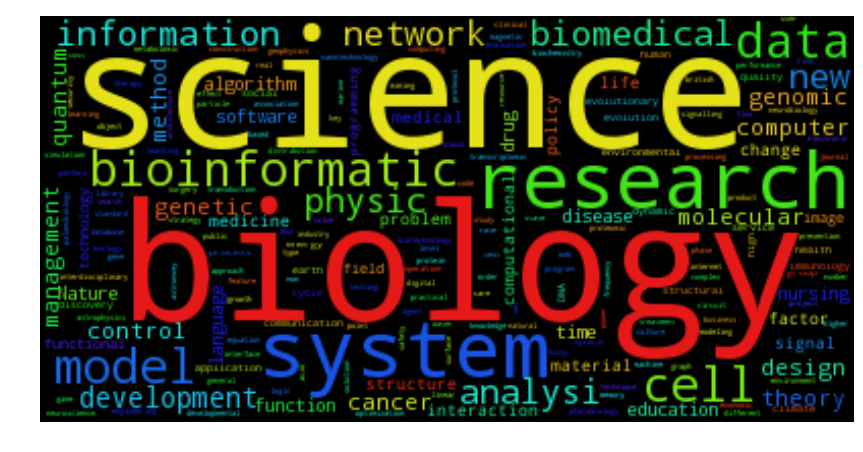
\includegraphics[width=16cm,height=7cm]{visual-gen}
    \caption{Most prominent general topics}
    \label{fig:topic}
\end{figure}
\begin{figure}[h]
    \centering
    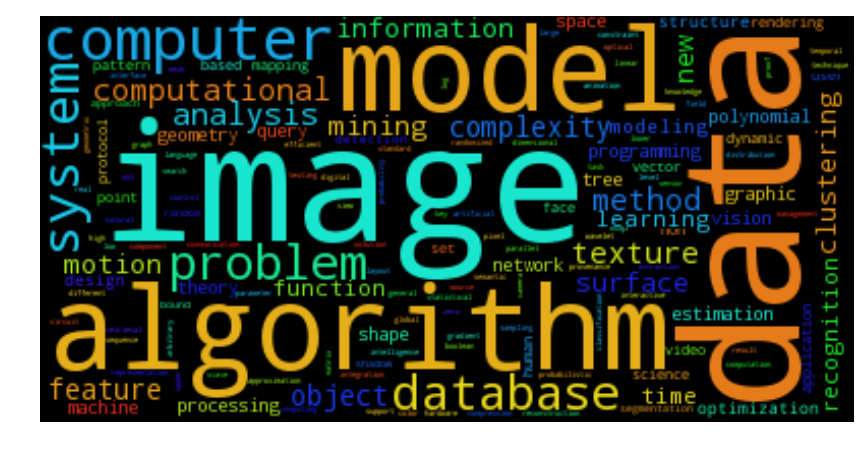
\includegraphics[width=16cm,height=7cm]{venue-image}
    \caption{Most prominent topics in computer science}
    \label{fig:venue}
\end{figure}


\section{Interesting visualizations of the dataset}
As our dataset has keywords of the academic papers as one of the attributes, we try to plot the histogram of the keywords presented in the dataset. In particular, we plotted two wordclouds: \\

1) General bag-of-words representation of the keywords of all the papers (Figure-\ref{fig:topic}). It can be seen from the figure that the research on biological topic is really cutting-edge and lot of academic papers are coming on the similar topics. \\
 
2) Histogram of keywords of famous computer science papers (which are published in top conferences/journals such as CVPR, SIGGRAPH, FOCS, KDD, SIGMOD (Figure-\ref{fig:venue}). Here, we can see that image processing, data mining and machine learning seem to be hot topics in computer science research.


\section{Social behavior of scientific papers}
A paper can be related to another paper through various different ways. For example, 1) one paper cites another paper. 2) Both papers cite some common paper. 3) They are accepted in the same journal/conference. 4) They can have the same authors etc. We can use these relationships to form a network or graph of papers. When we think of scoring these papers we can say that score of a paper will be dependent on scores of the papers it is connected to in this citation graph. Since there is an intutive correlation between scores of connected papers, when we have a new paper we can score it by looking at the scores of the papers it is connected to. In this way, network of papers behaves similar to any social network. This relationship allows us to apply recent developments in social relational learning \cite{deepwalk}, \cite{tang2011leveraging} to our problem. Also it allows us model our problem as a relational learning problem \cite{tang2009scalable}, \cite{tang2009relational}. 
\section{Approach}
The basic approach that will be used in scoring papers is given in Algorithm \ref{alg:algo1}
\begin{algorithm}
\caption{ - High level algorithm to get ranks of papers}
\label{alg:algo1}
\begin{algorithmic}[1]
\State Create a graph of papers capturing relations such as citations, authors, conferences etc.
\State Get latent social embeddings for the vertices of this graph. 
\State Create train and test data using some helper ranking function.
\State Train a model on this embedding to predict the score/rank of paper.
\end{algorithmic}
\end{algorithm}
Now, we will explain the algorithm in detail. Step-1 of the algorithm is trivial for our baseline model. We have created the graph using just citations as a criteria to get the citation graph of papers. We can easily extend this graph to include other relationships also as we have the necessary data to build such graph. Figure \ref{fig:datamodel} shows the fields we have for all the papers.


\begin{figure}[h]
    \centering
    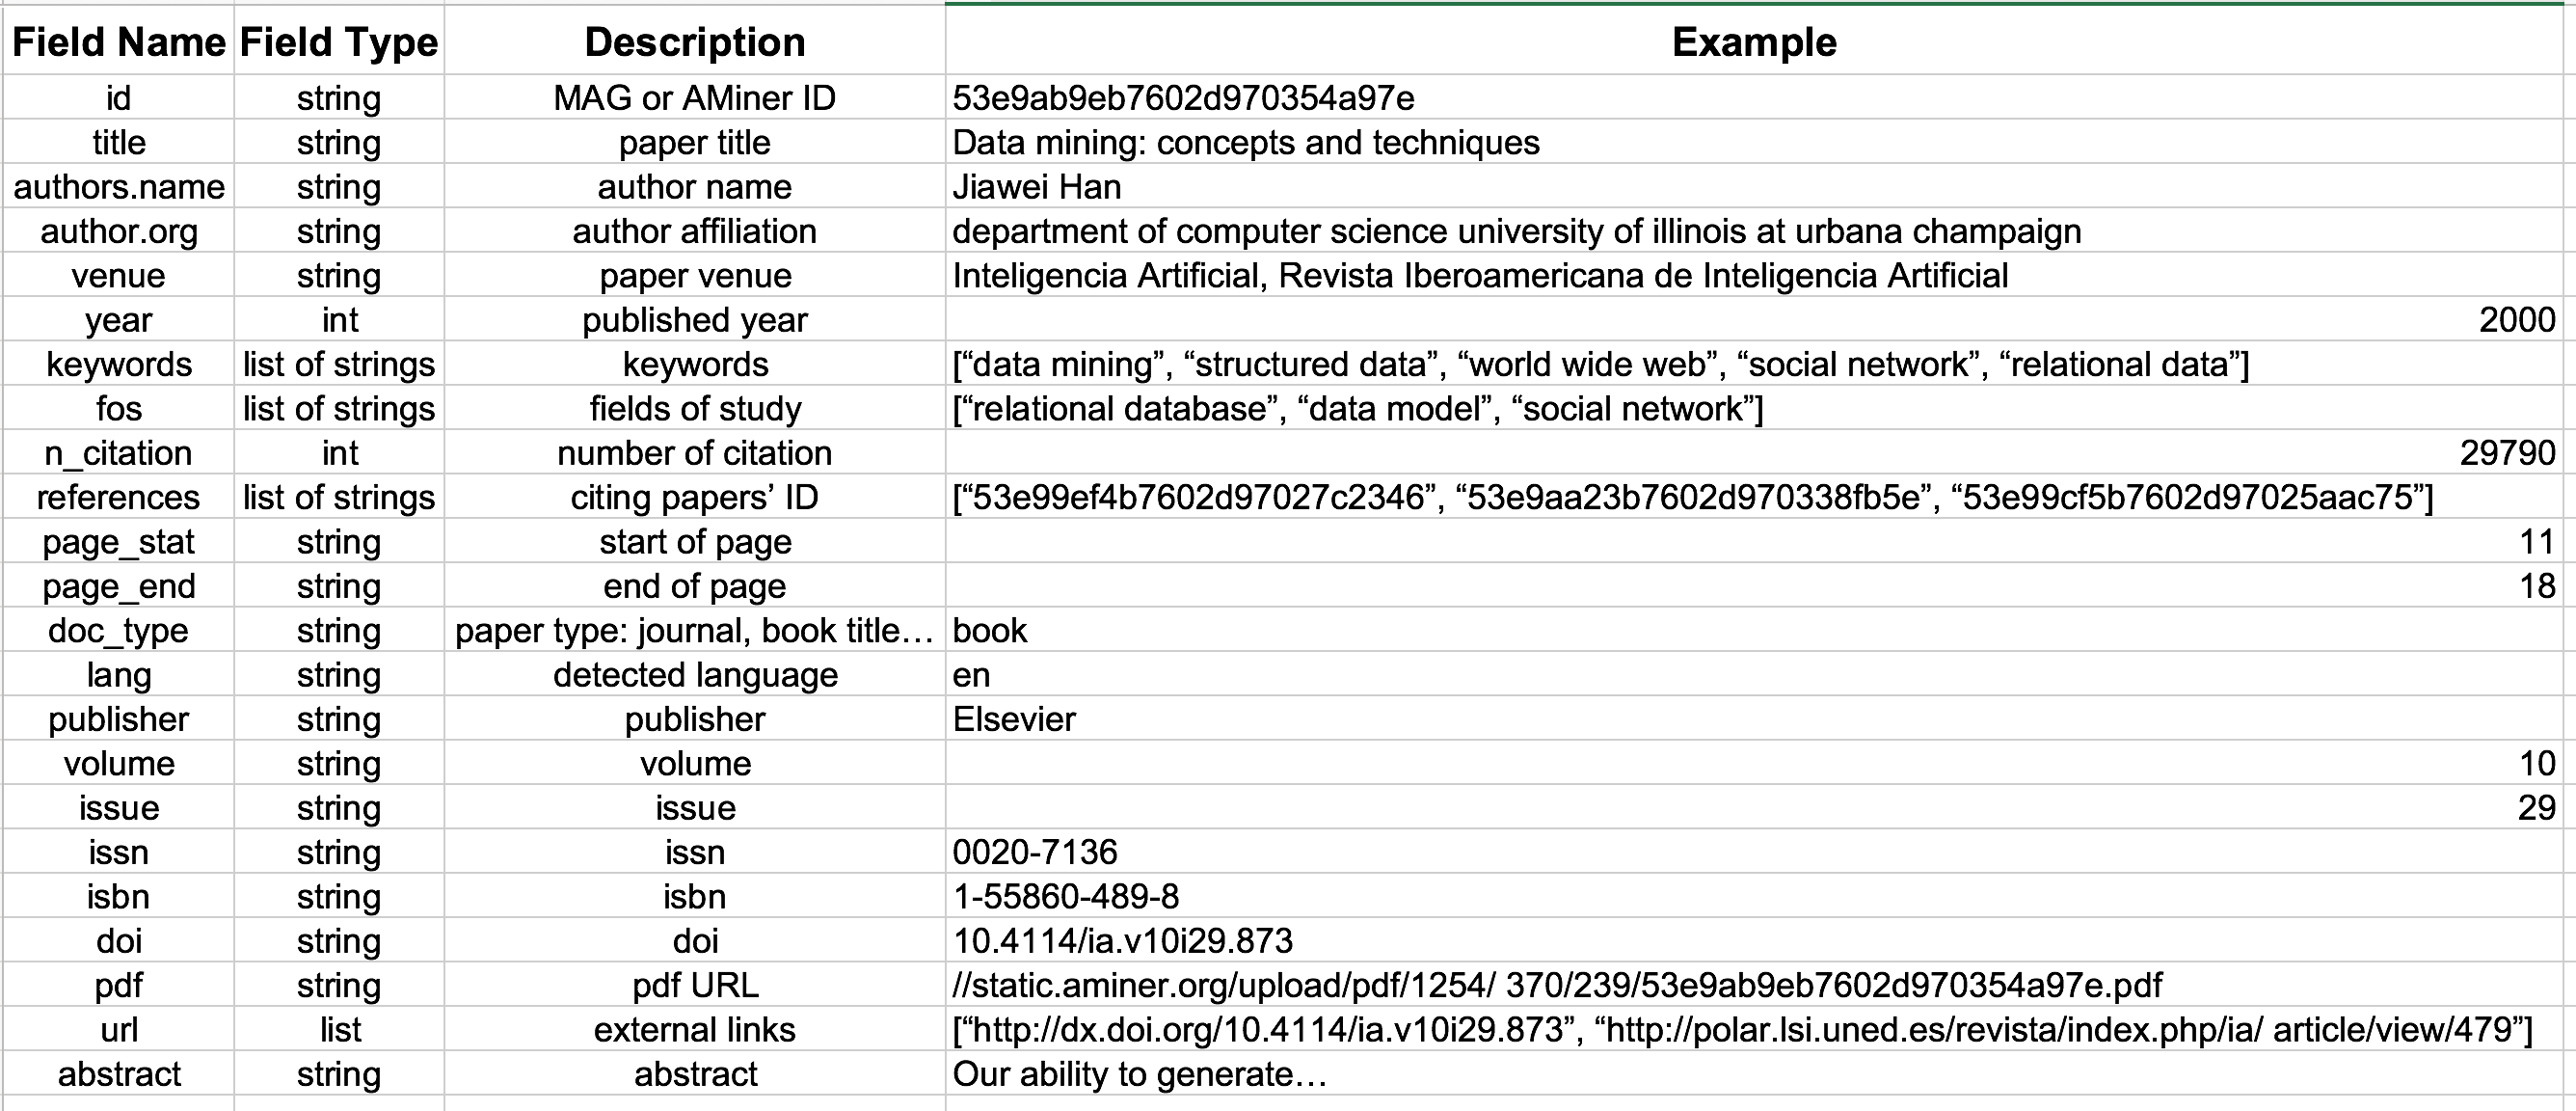
\includegraphics[width=17cm,height=8cm]{datamodel_new}
    \caption{Paper data model and its fields \cite{data}}
    \label{fig:datamodel}
\end{figure}


\subsection{Latent social representation of graph}
In the step-2 of our algorithm \ref{alg:algo1}, we need to get the latent social representation of the graph we constructed in step-1. We have used "DeepWalk" algorithm presented in \cite{deepwalk} to get the social embedding of the citation graph. "DeepWalk" applies deep learning techniques to learn the latent social representations of each vertex in the network. To achieve this,  \cite{deepwalk} presented an idea that random walks in a graph is similar to short sentences in a special language whose vocabulary is the set of vertices of the network. Hence, we can apply the same deep learning techniques that are used in natural language models to learn latent representation of each vertex. We will be using the same algorithm to get the representation of each vertex in our citation graph. There are other methods to get the social representation of a vertex such as Spectral clustering\cite{tang2011leveraging} which uses spectral graph theory(eigen values of Laplcian of graph), \cite{tang2009relational} uses eigen values of Modularity matrix of graph etc. Deepwalk works well on all types of  graphs and works very well even if the graph is sparsely labeled in relational classification task \cite{deepwalk}, which is exactly the kind of representation we would need to rank the papers as we have a very large graph( ~ 166 million vertices) with very sparse labeling (as we will be using experts to rank few papers). 
\subsection{Intuitive Ranking Helper Function}
We don't have any intuitive way to rank or score papers based on social representations we got from running DeepWalk on the graph. Also, it is very difficult to get a generalized scoring/ranking function that works universally well. But if we just consider a single feature out of all the possible parameters to decide if a paper is good or not, then we can have an intuitive ranking function that we can easily explain. Evidently, this ranking function does not generalize well. In this project,  we generalize this naive but intuitive ranking function by training some regression model on latent social representation of the graph. For baseline, we are considering a naive function that ranks a paper based on the conference or journal it was accepted in.  We can easily get the impact factors of conferences and journals. We assume that if a venue at which paper is published is good then paper is as good as the venue itself - the score of the paper is the same as the score of the venue. Using this naive intuitive function, we can sparsely get the scores of some of the papers in our graph. We can then train a regression model on this data to generalize the ranking function to look at the other aspects of the paper as well. In our base line model, graph is constructed using citations and our ranking helper function is only considering conferences that these papers were published in. 
\subsection{Prediction of the score/rank of a paper} 
To rank/score the papers, our initial approach was to get the feature vectors from deepwalk and then come up with a function of this feature vector to get a score of the paper. But after getting these feature vectors for each paper, we came to conclusion that its very hard to interpret what each of this dimension represents intuitively. So it was hard to come up with a function which would make sense and give us good results for all the papers using the feature vectors generated by DeepWalk. We believe we have a powerful tool in our hand in the form of these feature vectors we got from deepwalk, and we want to utilize its full potential. So, we tried to model ranking as a regression problem. Let's say we have ranks/scores of some of the papers. Now, we can easily train a model on the feature vectors to predict the rank or score of the rest of the papers. And as show in deepwalk, such model works well even in very sparsely labeled dataset such as YouTube \cite{deepwalk}.  So, for our baseline model, we ranked few papers manually.  We have used the ranks of conferences or journals to get an estimate on the rank/score of a paper that was published in that particular conference/journal. We have made an assumption that if conference/journal is good, then paper accepted in that journal/conference will be a good paper too. We used this logic to create the scores of papers in our training dataset for our models.
\section{Baseline model and Evaluation}
Our main goal of baseline model is to test whether our approach presented in algorithm \ref{alg:algo1} is correct or not. Also we wanted to test how accurately does the representations from deepwalk capture relationships not implicitly used in building the graph. To answer both these questions, we created our baseline model by creating a graph using citations of a paper (i.e. there will be an edge from paper A to paper B if B cites paper A). Note that the citation graph we consider here is a directed graph. We designed our helper ranking function naively by assuming that a paper is as good as venue it is published in. Using these sparsely labeled papers, we trained a linear regression model on the feature vectors we got by running DeepWalk on our graph. Algorithm \ref{alg:algo2} gives detailed algorithm for baseline model.
\begin{algorithm}
\caption{ - Algorithm for Baseline model}
\label{alg:algo2}
\begin{algorithmic}[1]
\State Create graph $G(V,E)$ using citations.
\State $G_{train}, G_{test}$ = Split($G$) (i.e. get random papers from graph to create training and testing datasets)
\State Intuitive\_ranking\_helper\_function($V_{train}$)
\State Intuitive\_ranking\_helper\_function($V_{test}$)
\State Initialize F as an array of feature vectors
\State F = DeepWalk(G) (This runs deepwalk on citations graph to get vector representation of each vertex)
\State $model$ = LinearModel($G_{train},F$) (Initialize a linear model)
\State Evaluate  $model$ on $G_{test}$
\State ranks = model.predict(G)
\State return ranks
\end{algorithmic}
\end{algorithm}
\begin{algorithm}
\caption{ - Algorithm for intuitively ranking papers}
\label{alg:algo3}
\begin{algorithmic}[1]
\Procedure{Intuitive\_ranking\_helper\_function}{$V$}
\State Initialize VenueRank table (this table has ranks of each conference and/or journal)
\For {$v$  in $V$}
	\State $rank[v] = rank[Venue[v]]$ (Naive way to rank the paper - paper is as good as the conference/journal it is published in)
\EndFor
\State return $rank$
\EndProcedure
\end{algorithmic}
\end{algorithm}

Now we will present the results of our experiment. 
\subsection{Experiment}
We have a data set consisting of 166,192,182 papers which is a huge number to deal with for a baseline model. So, we decided to limit ourselves to papers just in computer science field. We have selected total of $10,000$ papers for this phase of the project. We divided this dataset into $70\%$ training and $30\%$ testing splits. Table \ref{table:1} shows the results of our experiments. It can be seen that we have got $14\%$ error on our test datasets. Considering the facts - A) we constructed the graph using just citations and B) ranking function used for training was completely based on the ranks of conferences, we think this is an impressive result for a baseline model. Figure \ref{fig:errorhistogram} shows the histogram of errors for our model. It shows scores given by our model varies within 1 or 2 points of actual score. This is desirable property for our model as we want the model to generalize and take in to consideration other affiliations of the paper as well while scoring. $R^2$ value of our model is $0.095534$, which is indicates that our model might not be that good and can be improved. Figure \ref{fig:ptest} shows the p-test result for our model. Our p-value is 0.043, which indicates that our model is good and we can reject the null hypothesis.  \\
\\From the evaluation of our model, it is clear that the hypothesis we made is actually true. We can say that the approach we are using works and we can make further progress by improving our model to get better results. We have also shown that "DeepWalk" indeed captures the relationships which are not explicit at the time of creation of graph. We created the graph using citations and still got good results when we trained the model to basically predict the relationship based on conferences. 

\begin{table}[h!]
\centering
\begin{tabular}{||c c c ||} 
 \hline
 Data Set & Training &  Testing \\ [0.5ex] 
 \hline\hline
 Mean Error &  15.03 \%& 13.97\% \\ [1ex] 
Median Error & 13.8\%  & 13.87\% \\ [1ex] 
 \hline
\end{tabular}
\caption{Error rates for linear regression baseline model}
\label{table:1}
\end{table}
\begin{figure}[h]
    \centering
    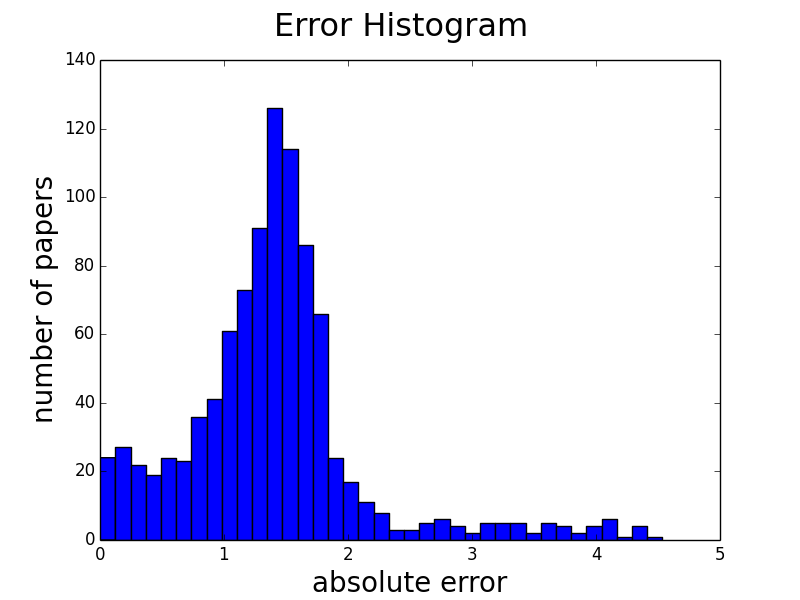
\includegraphics[width=17cm,height=11cm]{figure_1}
    \caption{Error histogram of baseline model}
    \label{fig:errorhistogram}
\end{figure}
\begin{figure}[h]
    \centering
    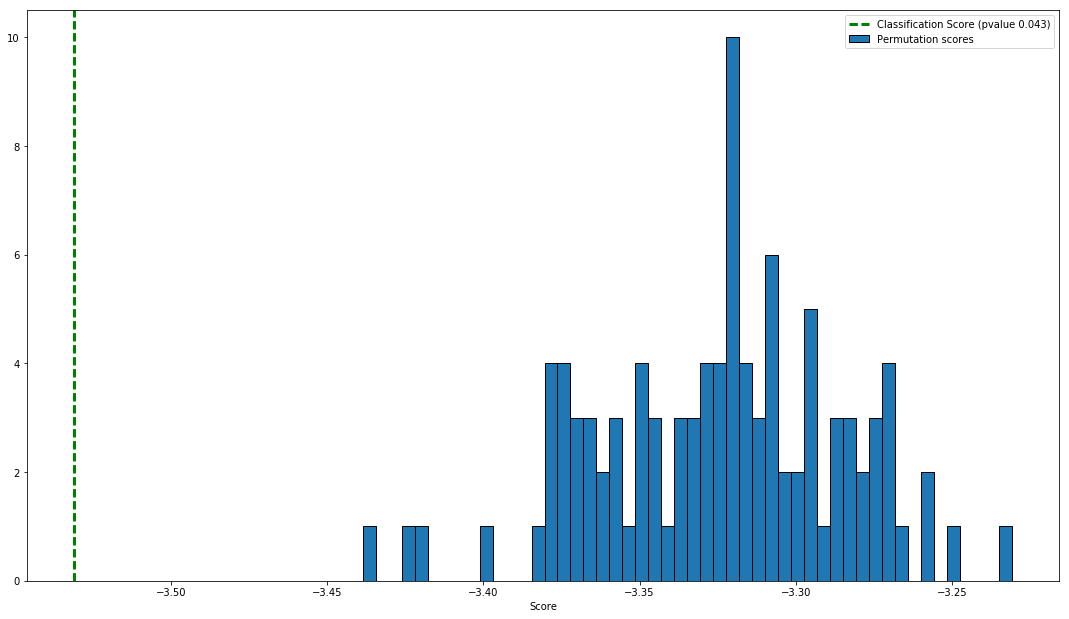
\includegraphics[width=16cm,height=9cm]{permutation_test}
    \caption{P-test for model}
    \label{fig:ptest}
\end{figure}
\section{Future Work and Conclusion}
From the results of the experiments, we can see that ranking function really depends on our helper function and the graph we constructed using papers. We can see now a few ways to improve our model.
\begin{enumerate}
\item Instead of using a helper function we can get an expert to rank or we can rank ourselves, a small number of papers. So, we get a more robust initial estimate of ranks of papers. We think this kind of function will generalize better using our approach.
\item We can construct graph using various other homophily such as authors, conferences etc. We believe that the more relationships we capture in our initial graph, the better results we can get for the papers which do not have all the information such as citations, conferences etc.
\item We can also improve our model by using non-linear regression model in the last step of our algorithm.
\end{enumerate}
We will try above approaches in an attempt to improve our baseline model. Intuitively, we feel that we can get better results if we combine the training of DeepWalk and regression linear model together, similar to the deep learning models used in NLP tasks. And if time permits we want to try this approach as well. The implementation of this approach will certainly require deep understanding of DeepWalk algorithm at coding level.

\begin{thebibliography}{9}
\bibitem{deepwalk}
Perozzi, B. ,Al-Rfou, R.,Skiena, S.
\newblock DeepWalk: Online Learning of Social Representations
\newblock Proceedings of the 20th ACM SIGKDD International Conference on Knowledge Discovery and Data Mining
\newblock KDD '14
\bibitem{tang2009relational}
Tang, Lei and Liu, Huan
\newblock Relational learning via latent social dimensions
\newblock Proceedings of the 15th ACM SIGKDD international conference on Knowledge discovery and data mining,2009



\bibitem{tang2009scalable}
Tang, Lei and Liu, Huan
 \newblock Scalable learning of collective behavior based on sparse social dimensions
  \newblock Proceedings of the 18th ACM conference on Information and knowledge management,2009
\bibitem{Hirsch}
J. E. Hirsch.
\newblock An index to quantify an individual's scientific research output, 2005,
\newblock Proc.Nat.Acad.Sci.46:16569,2005;
\newblock arXiv:physics/0508025.
\newblock DOI: 10.1073/pnas.0507655102.
\bibitem{gindex}
Egghe, L.
\newblock  Theory and practise of the g-index
\newblock Scientometrics (2006) 69: 131.
\newblock https://doi.org/10.1007/s11192-006-0144-7
\bibitem{pagerank}
Page, L., Brin, S., Motwani, R., Winograd, T. 
\newblock  The PageRank citation ranking: Bringing order to the web  
\newblock  (Technical Report). Stanford InfoLab.
\bibitem{garfield}
Garfield, E.
\newblock  Citation analysis as a tool in journal evaluation
\newblock Science,178,471-479.
\bibitem{pinski}
Pinski, G.,  Narin, F. 
\newblock Citation influence for journal aggregates of scientific publications: Theory, with application to the literature of physics
\newblock  Information Processing and Management, 12(5), 297-312
\bibitem{data}
Microsoft Academic Graph 
\newblock https://www.openacademic.ai/oag/
\bibitem{arxiv}
arXiv.org
\newblock  https://arxiv.org/


\bibitem {tang2011leveraging}
  Tang, Lei and Liu, Huan
  \newblock Leveraging social media networks for classification
  \newblock Data Mining and Knowledge Discovery,2011,Springer
 
\end{thebibliography}

\listoffigures
\end{document}